% chapters/chapter3/3_5_nmpc_traj.tex
% !TeX root=../../main.tex

\section{ارزیابی \lr{NMPC} در ردیابی مسیر}
\label{sec:nmpc_traj_analysis}

همان‌گونه که در ارزیابی بخش پیشین مشاهده شد، فقدان یک مسیر مرجع پیوسته (\lr{Trajectory}) و مواجهه مستقیم کنترل‌کننده با یک خطای موقعیت بزرگ، سیستم را به سرعت به سمت مرزهای قیود فیزیکی (هم در نیروی ارابه و هم در کران‌های زاویه آونگ) سوق داد. درگیری ممتد با این مرزها برای حفظ پایداری، به نوسانات شدید و نامطلوب در نیروی کنترلی اعمالی انجامید. برای رفع این چالش بنیادین، در این بخش معماری یکپارچه‌ای ارزیابی می‌شود که در آن، برنامه‌ریز مسیر سینماتیکی آرایه‌ای از نقاط مرجع آینده را تولید کرده و به افق پیش‌بینی \lr{NMPC} تزریق می‌کند. این آگاهی پیش‌دستانه (\lr{Proactive}) به حل‌گر اجازه می‌دهد تا تلاش کنترلی را در طول زمان توزیع کرده و از بروز رفتارهای تهاجمی جلوگیری کند.

\subsection{مانور کوتاه‌برد}
در سناریوی نخست، کالسکه برای طی کردن مسافت $0.5$ متر تحت هدایت این معماری قرار گرفت. پاسخ زمانی متغیرهای حالت در شکل~\ref{fig:nmpc_traj_05_states} حاکی از ردیابی بسیار دقیق موقعیت کالسکه ($x$) با حداقل خطای گذرا است. به دلیل وجود مسیر مرجع هموار، زاویه نوسان آونگ ($\theta$) به شدت سرکوب شده و در بیشینه خود از حدود $0.08$ رادیان فراتر نمی‌رود.

در این مانور، متغیر طول کابل ($l$) عملاً روی مقدار اولیه خود ($0.5$ متر) ثابت باقی مانده است. دلیل این امر آن است که در مسافت‌های کوتاه و شتاب‌گیری‌های ملایم، انرژی ارتعاشی قابل‌توجهی به پاندول تزریق نمی‌شود که نیازمند فعال‌سازی مکانیزم میرایی از سوی بهینه‌ساز باشد.

\begin{figure}[htbp]
    \centering
    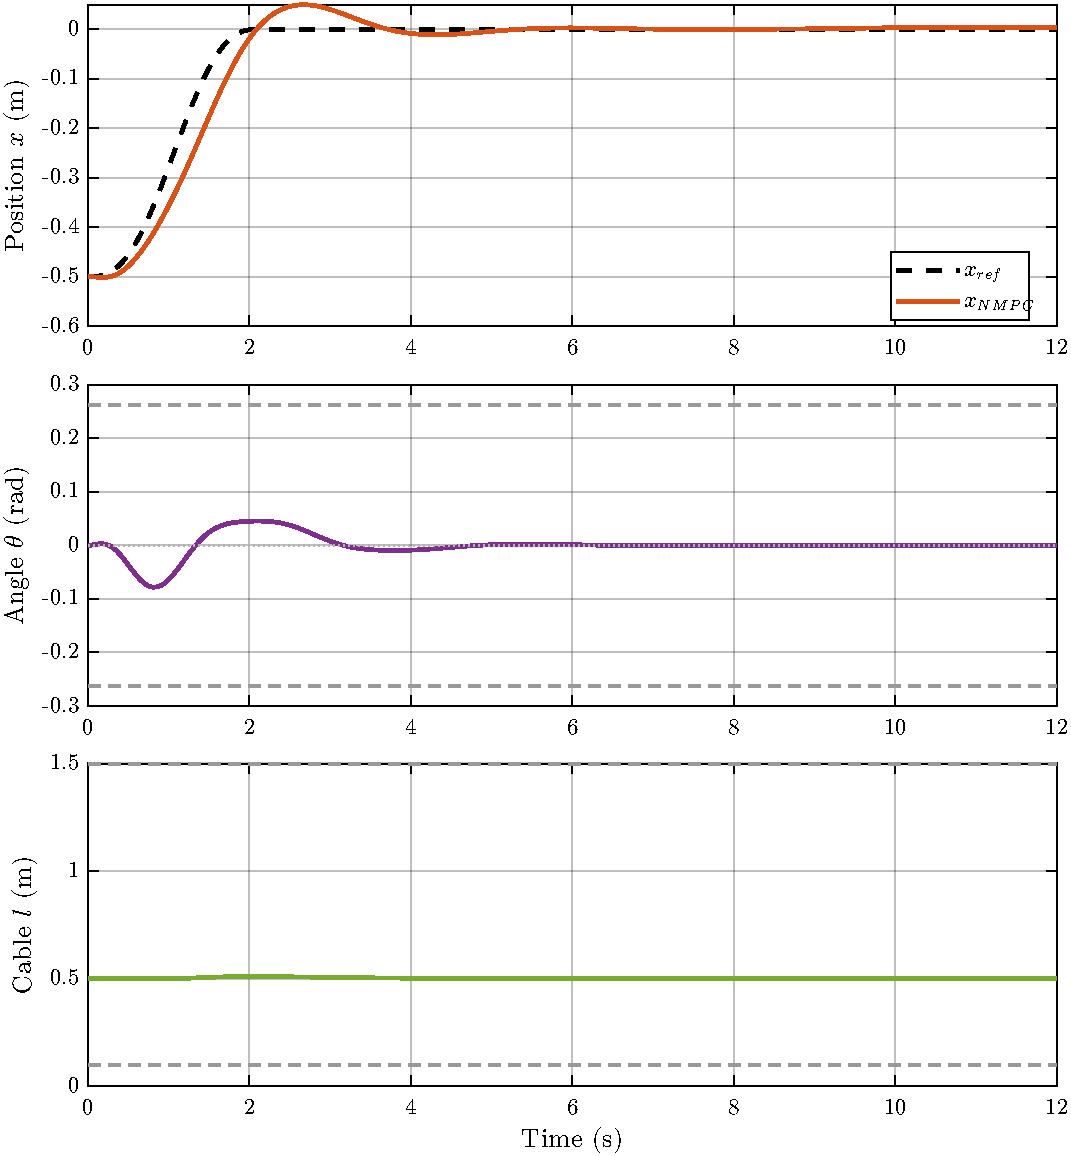
\includegraphics[width=0.75\textwidth]{images/4_NMPC_Trajectory/MPC_TRAJ_x_theta_l.pdf}
    \caption{\rl{پاسخ زمانی متغیرهای حالت در مانور $0.5$ متر؛ ردیابی دقیق و عدم نیاز به تغییر طول کابل.}}
    \label{fig:nmpc_traj_05_states}
\end{figure}

بررسی سیگنال‌های کنترلی در شکل~\ref{fig:nmpc_traj_05_inputs} نیز نشان‌دهنده یک رفتار کاملاً ایمن و هموار است؛ نیروی کالسکه در بازه بسیار کوچکِ کمتر از $1\,\mathrm{N}$ تغییر کرده و شتاب وینچ تقریباً صفر است که نشان از حذف کامل شوک‌های کنترلی دارد.

\begin{figure}[htbp]
    \centering
    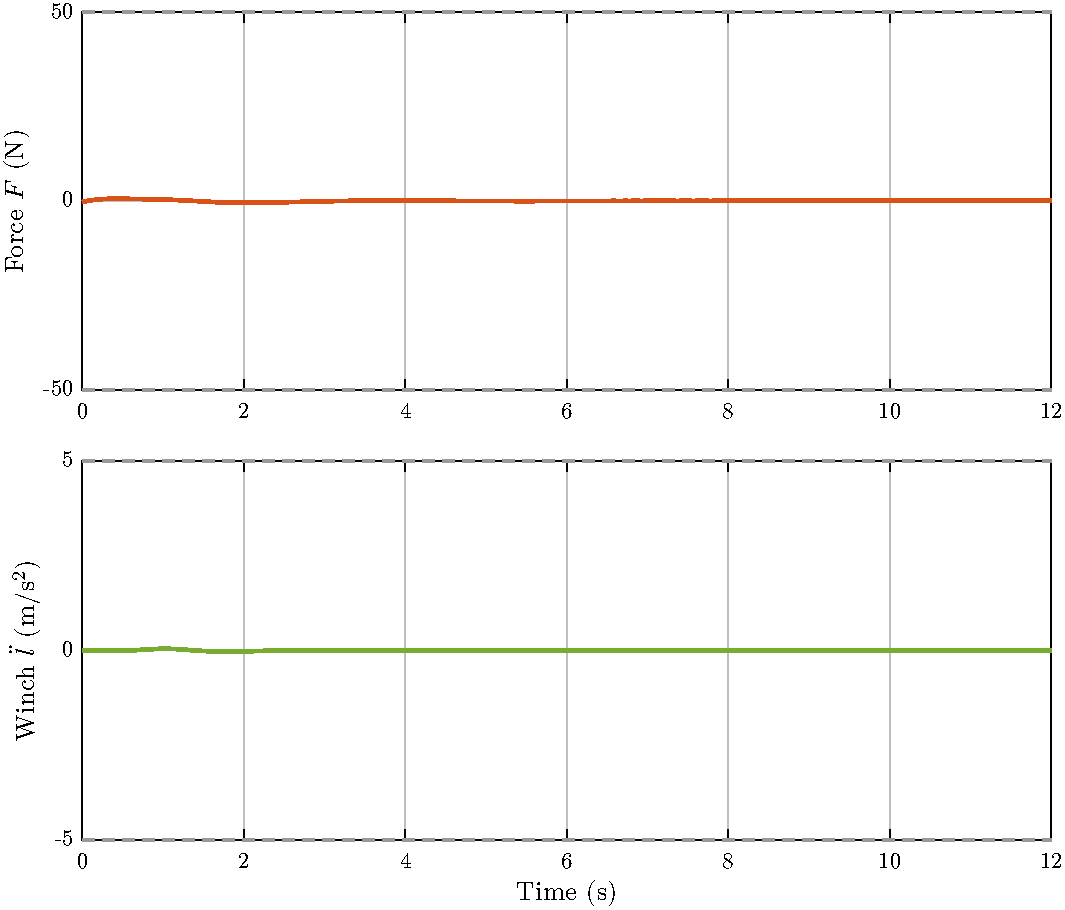
\includegraphics[width=0.75\textwidth]{images/4_NMPC_Trajectory/MPC_TRAJ_f_l_ddot.pdf}
    \caption{\rl{سیگنال‌های کنترلی در مانور $0.5$ متر؛ رفتار کاملاً هموار و توقف نوسانات نیرویی.}}
    \label{fig:nmpc_traj_05_inputs}
\end{figure}

\subsection{مانور بلندبرد}
اثربخشی واقعی معماری یکپارچه در مانور $5$ متری آشکار می‌شود. برای بررسی دقیق‌تر کیفیت هدایت، پاسخ ردیابی متغیرهای حالت نسبت به سیگنال‌های مرجع در شکل~\ref{fig:nmpc_traj_tracking_5} رسم شده است. همان‌طور که مشاهده می‌شود، موقعیت و سرعت کالسکه ($x$ و $\dot{x}$) با انطباق بالایی پروفایل سینماتیکی مرجع (منحنی‌های نقطه‌چین) را دنبال می‌کنند و چالش فراجهش‌های بزرگ که در پاسخ پله وجود داشت، کاملاً برطرف شده است.

در خصوص دینامیک آونگ، هدف کنترلی حفظ زاویه ($\theta$) و سرعت زاویه‌ای ($\dot{\theta}$) روی مرجع صفر است. نتایج نشان می‌دهد که کنترل‌کننده با موفقیت نوسانات فاز گذرا را در محدوده‌ای بسیار امن (بیشینه دامنه حدود $0.13$ رادیان) مهار کرده و از نزدیک شدن به کران بحرانی $\pm0.26$ رادیان جلوگیری می‌کند. مهم‌ترین دستاورد این بخش، هم‌گرایی کامل زاویه و سرعت زاویه‌ای به صفر در لحظه توقف کالسکه ($t=10\,\mathrm{s}$) است که به معنای حذف مطلق نوسان پسماند (\lr{Residual Sway}) است.

\begin{figure}[htbp]
    \centering
    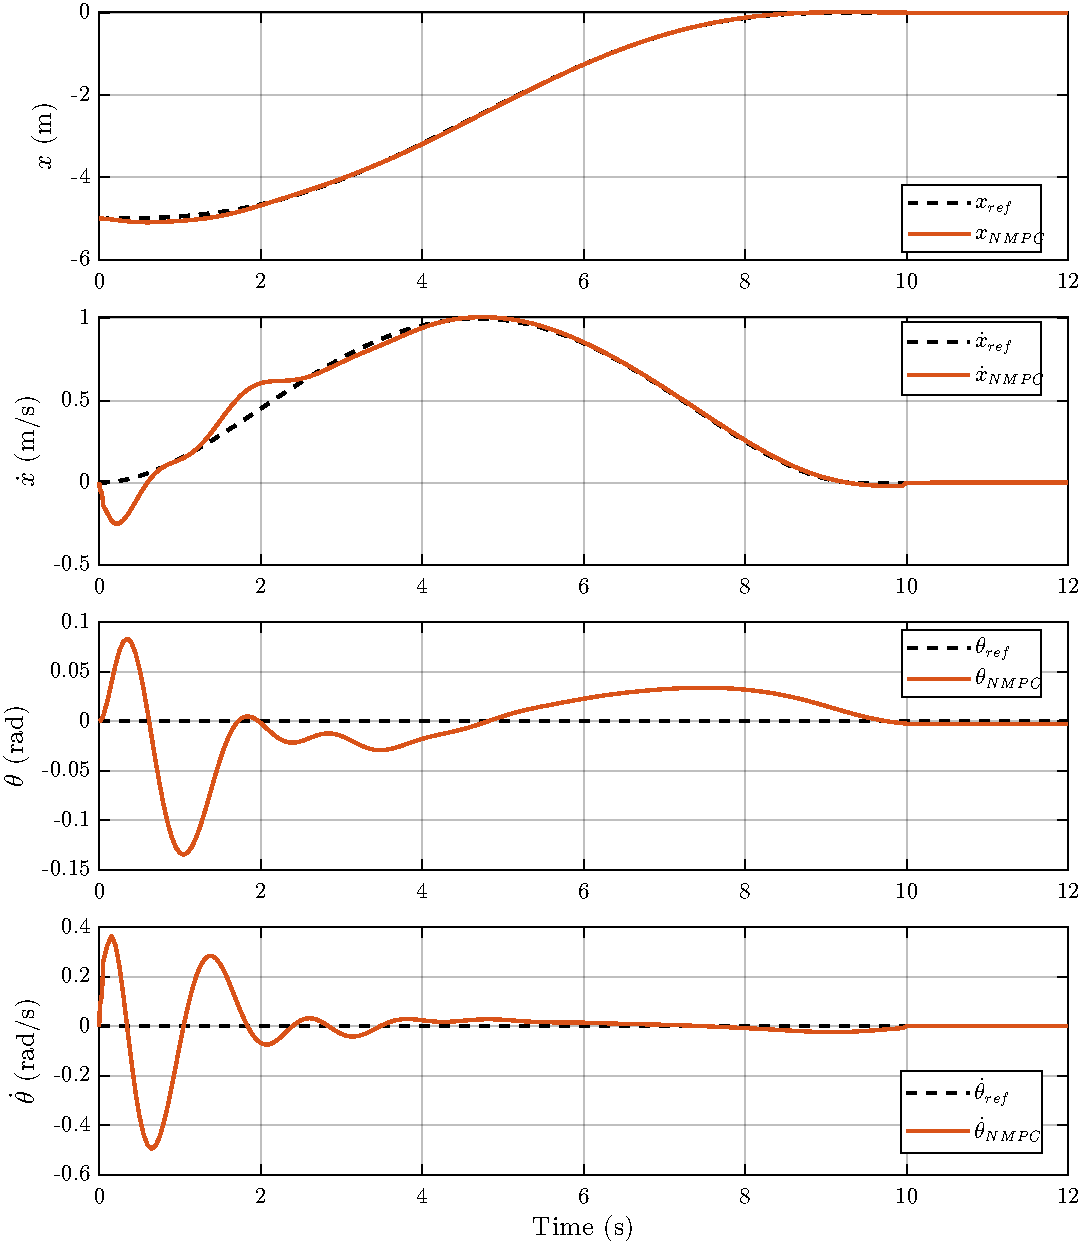
\includegraphics[width=0.85\textwidth]{images/4_NMPC_Trajectory/NMPC_TRAJ_StateTracking_5.pdf}
    \caption{\rl{جزئیات ردیابی مسیر در مانور $5$ متر؛ انطباق سرعت کالسکه با مرجع و هم‌گرایی زاویه آونگ به صفر در زمان توقف.}}
    \label{fig:nmpc_traj_tracking_5}
\end{figure}

\subsection{نقش تغییر طول کابل در کنترل نوسان}
بررسی رفتار متغیرهای حالت در شکل~\ref{fig:nmpc_traj_5_states} مکانیزم درونی حل‌گر برای سرکوب نوسان را روشن می‌سازد. در فاز میانی حرکت که کالسکه تحت شتاب‌های متغیر قرار دارد، طول کابل ($l$) از مقدار اولیه $0.5$ متر تا حدود $0.68$ متر افزایش می‌یابد و پیش از توقف کامل، مجدداً به طول تعادل بازمی‌گردد.

رفتار مشاهده‌شده با استفاده از تغییر طول کابل به‌عنوان یک درجه آزادی فعال برای مدیریت نوسان سازگار است. از منظر فیزیکی، افزایش طول کابل فرکانس طبیعی آونگ را کاهش داده و تمایل سیستم به جذب انرژی ارتعاشی از شتاب کالسکه را تضعیف می‌کند. حل‌گر \lr{NMPC} با بهره‌گیری از معادلات دقیق غیرخطی در افق پیش‌بینی، این مکانیزم سینماتیکی را به عنوان یک میراگر فعال به کار گرفته تا پایداری بار را در طول مسیرهای طولانی تضمین کند.

\begin{figure}[htbp]
    \centering
    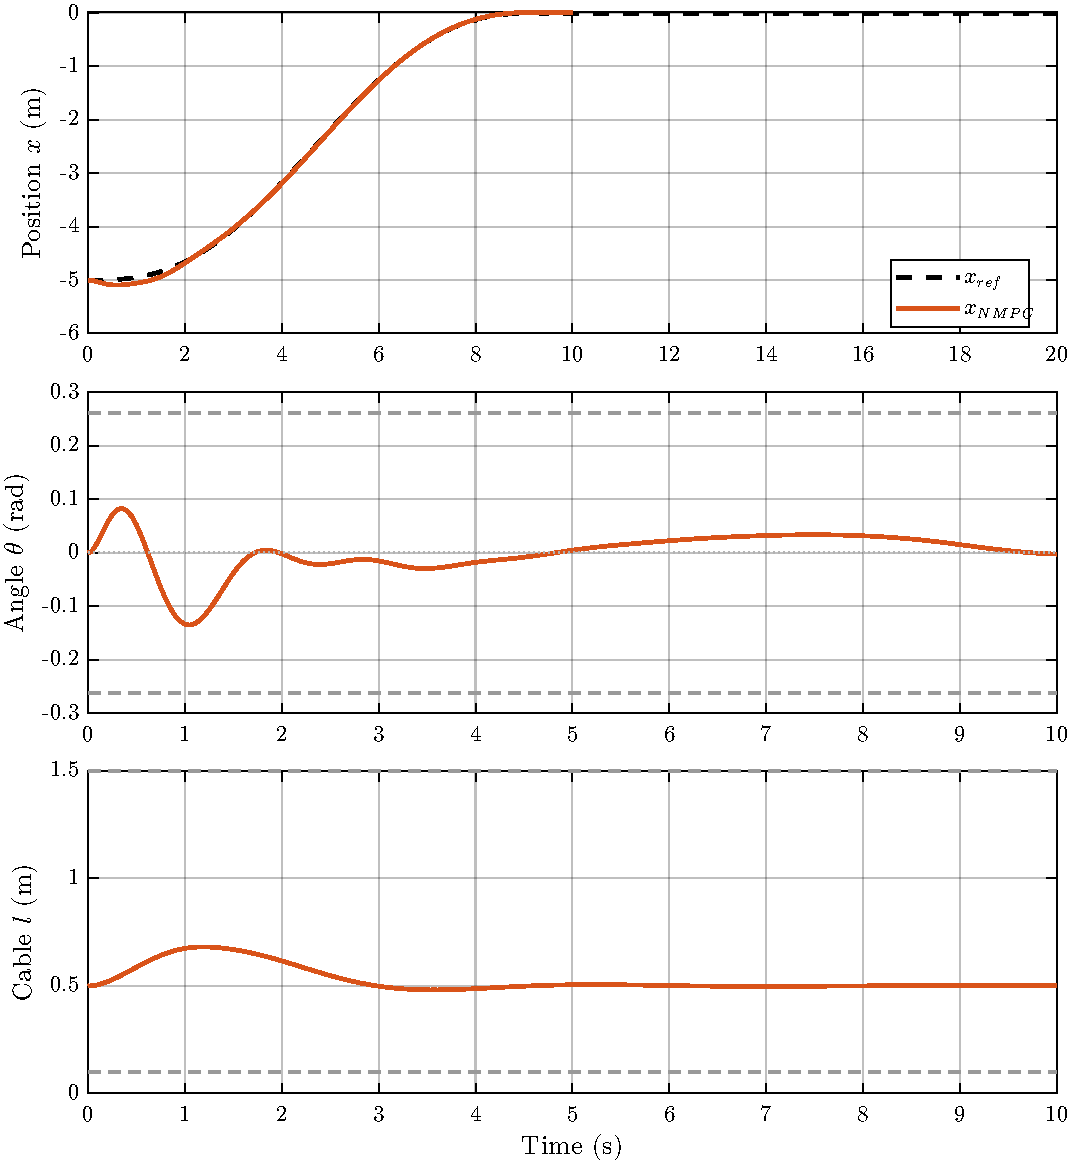
\includegraphics[width=0.75\textwidth]{images/4_NMPC_Trajectory/MPC_TRAJ_x_theta_l_5.pdf}
    \caption{\rl{پاسخ زمانی متغیرهای حالت در مانور $5$ متر؛ بهره‌گیری از انبساط کابل برای مدیریت نوسان پاندول.}}
    \label{fig:nmpc_traj_5_states}
\end{figure}

\subsection{قیود و تلاش کنترلی}
مشاهده پروفایل ورودی‌های کنترلی در مانور $5$ متری (شکل~\ref{fig:nmpc_traj_5_inputs}) تفاوت فاحش این معماری را با حالت پاسخ پله برجسته می‌سازد. نیروی اعمالی ارابه کاملاً هموار و پیوسته است و بیشینه آن از حدود $2.5\,\mathrm{N}$ تجاوز نمی‌کند. این مقدار نشان می‌دهد که سیستم با حاشیه امنیتی بسیار بزرگی نسبت به قید فیزیکی سیستم ($50\,\mathrm{N}$) فعالیت می‌کند (خطوط چین‌دار $\pm5\,\mathrm{N}$ در تصویر صرفاً برای نمایش مقیاس رسم شده‌اند).

همچنین متغیر شتاب وینچ ($\ddot{l}$) با دامنه‌ای کمتر از $1.5\,\mathrm{m/s^2}$ به صورت نرم تغییر می‌کند که به طور کامل قید فیزیکی عملگر کابل ($5\,\mathrm{m/s^2}$) را ارضا می‌نماید. حذف کامل نوسانات فرکانس بالا (\lr{Chattering}) و درگیری‌های مرزی، اثبات می‌کند که تزریق مسیر مرجع به کنترل‌کننده پیش‌بین، نه تنها کیفیت ردیابی را ارتقا می‌دهد، بلکه رفتار دینامیکی عملگرها را به سطحی مطلوب برای کاربردهای واقعی و صنعتی می‌رساند.

\begin{figure}[htbp]
    \centering
    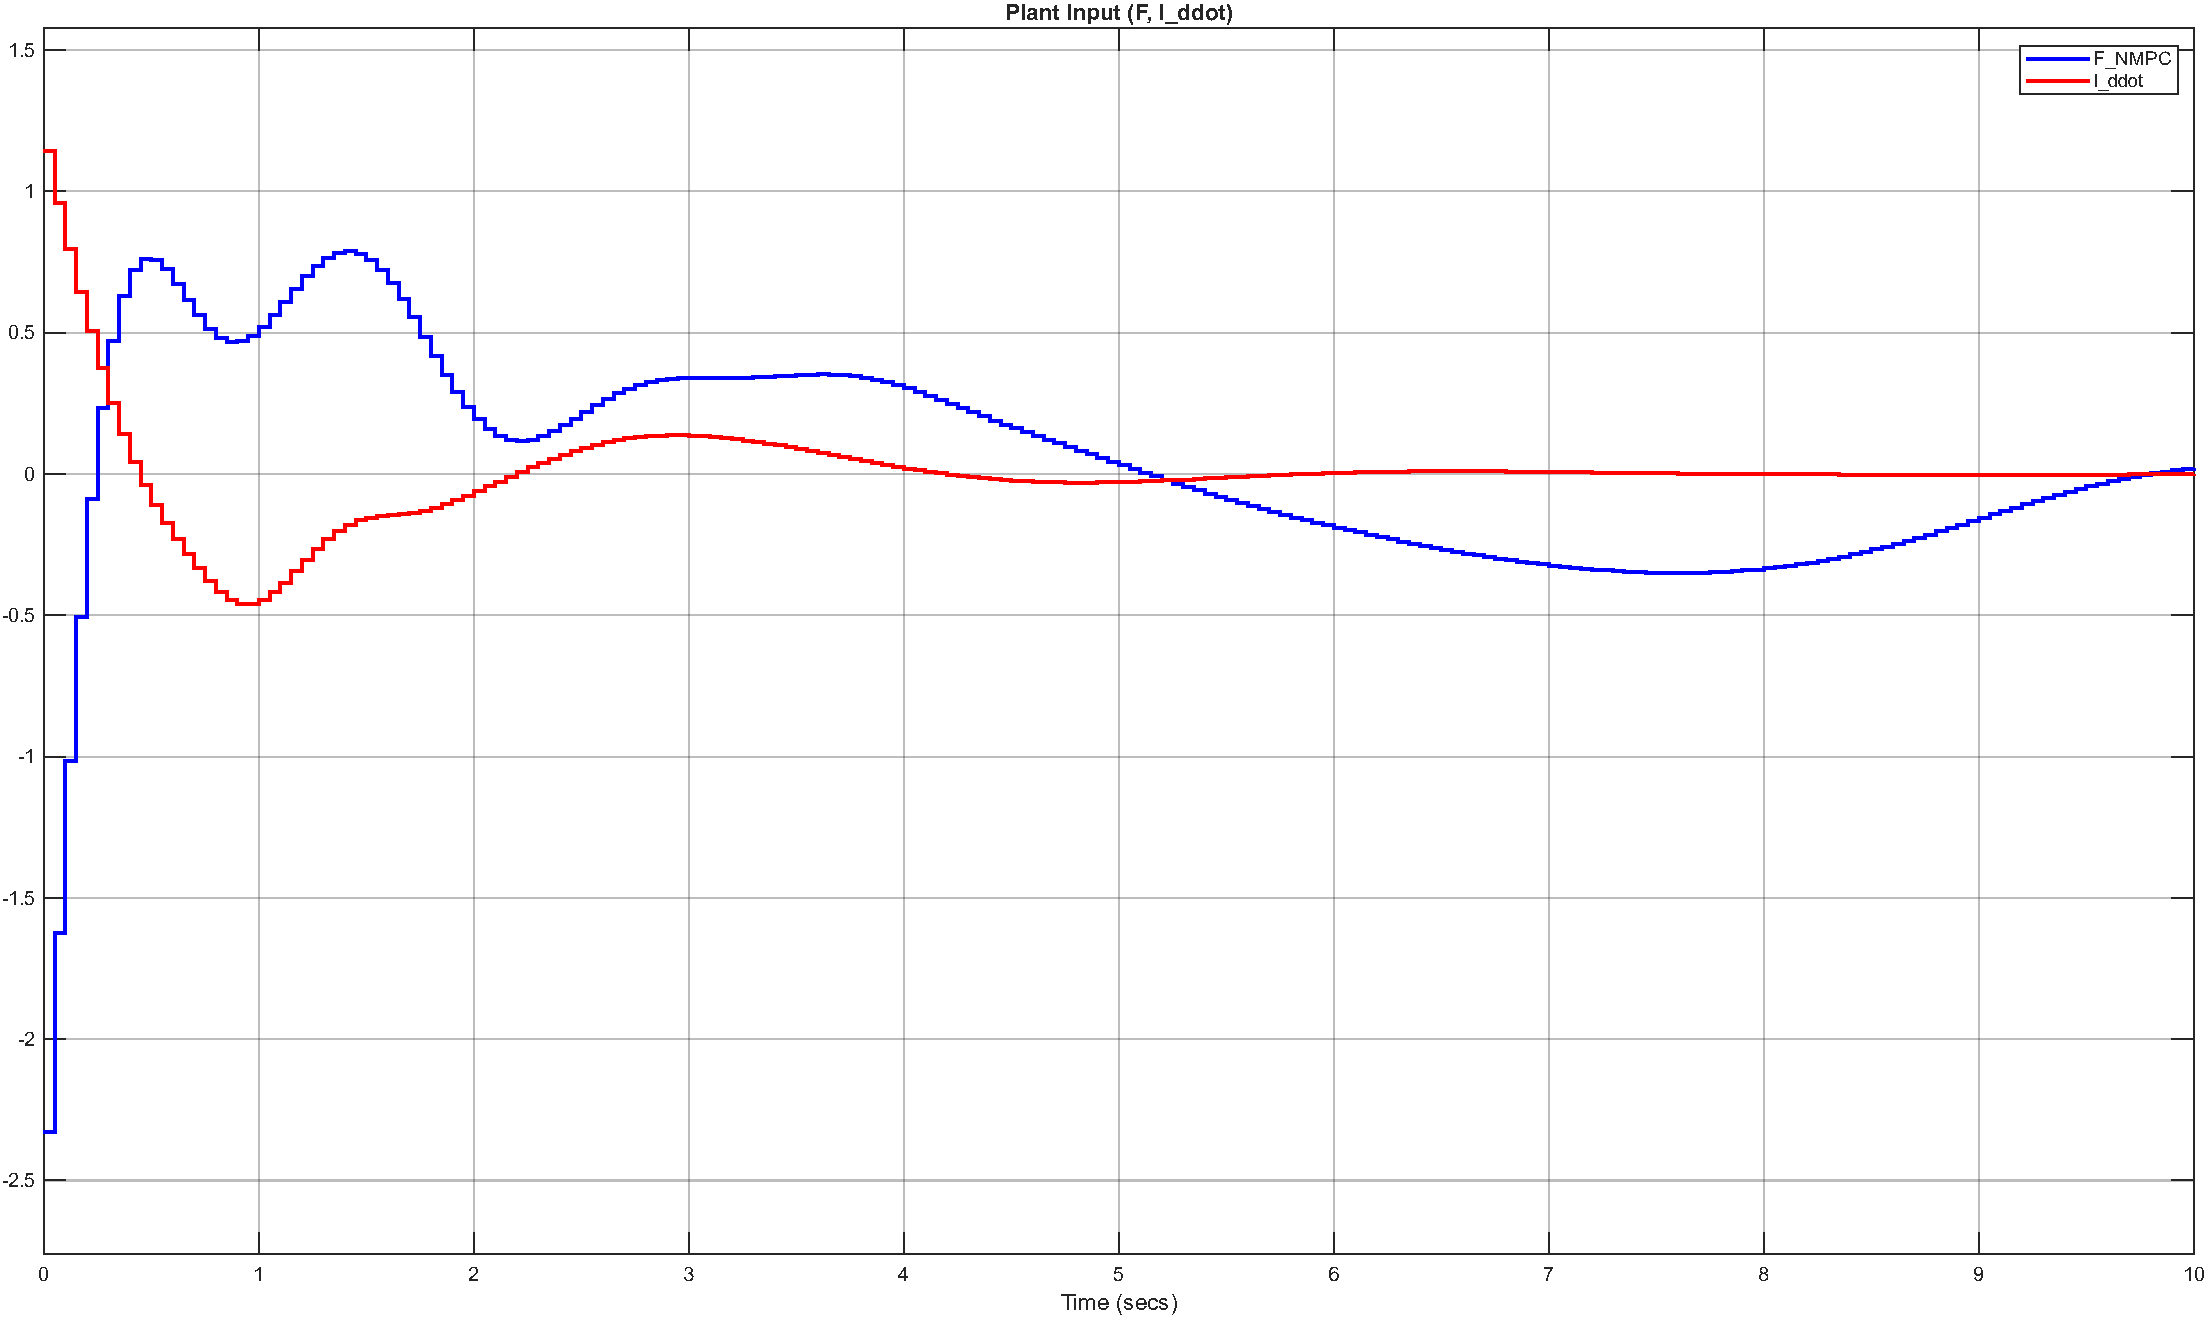
\includegraphics[width=0.75\textwidth]{images/4_NMPC_Trajectory/MPC_TRAJ_f_l_ddot_5.pdf}
    \caption{\rl{تلاش کنترلی در مانور $5$ متر؛ ارضای کامل قیود فیزیکی و حذف رفتار نوسانی فرکانس بالا.}}
    \label{fig:nmpc_traj_5_inputs}
\end{figure}